\title{LEZIONE 18 20/05/20}
\textbf{link} \href{https://web.microsoftstream.com/video/71a20262-9f5a-4991-8c41-af0a21825730?list=user&userId=cfe0965d-9a7c-40e2-be6e-f078296a1914}{clicca qui}
\subsection{AJAX: javascript e l'interazione client server asincrona}
L'architettura fat client permette di separare (rendere asincorna) l'interazione dell'utente col browser da quella del browser (client) col server e di evitare il ricarico completo dell'interfaccia.\newline
\newline
Uno script può richiedere al browser l'invio di una richiesta HTTP e la ricezione (asincron) della risposta.\newline
XMLHttpRequest è un'interfaccia che permette ddi creare oggetti (normalmente gestiti dal browser) utili per:
\begin{itemize}
    \item inviare richieste HTTP (o HTTPs) ad un web server;
    \item Restituire i dati provenienti dalla risposta del server allo script.
\end{itemize}
L'oggetto globale window contiene l'oggetto di utilità XMLHttpRequest che è, in poche parole, l'interfaccia di rete del browser.\newline
\newline
L'oggetto XMLHttpRequest possiede uno stato, attributi e metodi e può generare eventi.\newline
La caratteristica principale è proprio il suo stato che evolve nel tempo e che descrive l'avanzamento della richiesta HTTP. gli stati ammissibili sono:
\begin{itemize}
    \item UNSENT = 0;
    \item OPENED = 1;
    \item HEADERS\_RECEIVED = 2;
    \item LOADING = 3;
    \item DONE = 4.
\end{itemize}
Gli attributi principali sono invece:
\begin{itemize}
    \item readyState: memorizza lo stato corrente del processamenteo della richeista; ha come valori i possibili stati elecanti prima;
    \item onreadystatechange: memorizza lafunzione che gestisce l'evento dicambio dello stato (event handler);
    \item upload: memorizza un oggetto di tipo XMLHttpRequestUpload che permette di monitorare lo stato di richieste che comprendono un body;
    \item status, statusText: memorizza lo status code e message della risposta HTTP;
    \item response, responseText, responseXML: memorizza il contenuto (body) della risposta.
\end{itemize}
I metodi principali sono:
\begin{itemize}
    \item open(metodo, url) oppure open(metodo, url, asyncFlag, username, pwd): permettono di creare una richiesta con metodo specificato indirizzata a un URL specificato; per default la richiesta è asincrona.
    \item setRequestHeader(nome, valore): permette di assegnare valore a header della richiesta;
    \item send(body-opzionale): effettua l'invio della richiesta HTTP, opzionalmente allegando un request body;
    \item abort(): interrompe la richiesta.
\end{itemize}
Gli eventi principali sono:
\begin{itemize}
    \item readystatechange: generato quando l'attributo readyState cambia valore, è l'evento più usato e più importante;
    \item loadstart, progress, abort, error, load, timeout, loadend: altri eventi meno usati, l'evento readystatechange permette già di gestire tutti i casi, questi eventi sono più moderni e specifici, ma non sono supportati da tutti i browser.
\end{itemize}
\ \newline
Inviare una richiesta asincrona non è un lavoro difficile, basta usare i metodi open e send dell'oggetto XMLHttpRequest, gestire la risposta è invece la parte più complessa solitamente.\newline
Lo stato della richiesta può essere monitorato controllando le proprietà dell'oggetto XMLHttpRequest:
\begin{itemize}
    \item XMLHttpRequest.readyState mantiene traccia dello stato della richiesta;
    \item XMLHttpRequest.onreadystatechange contiene un riferimento a una funzione che viene chiamata ogni volta che XMLHttpRequest.readyState cambia, cioè si produce l'evento readystatechange;
    \item XMLHttpRequest.status permette di controllare l'esito, per esempio vale 200 quando la risposta è OK oppure 404 quando la risorsa richiesta non è stata trovata.
\end{itemize}
Il contenuto della risposta del serer si trova come valore della proprietà responseText o responseXML (c'è anche JSON: studio autonomo).\newline
\newline
Vediammo ora la tipica funzione che effettua la chiamata:
\begin{lstlisting}
    function makeCall(method, url, formElement, cback, reset=true){
        var req = new XMLHttpRequest();
        req.onreadystatechange = function(){
            cback(req);
        };
        req.open(method, url);
        if(formElement == null){
            req.send();
        }
        else{
            req.send(new FormData(formElement));
        }
        if(formElement !== null && reset === true){
            formElement.reset();
        }
    }
\end{lstlisting}
\ \newline
Vediamo ora un'immagine riassuntiva dell'architettura asincrona con XMLHttpRequest:
\begin{center}
    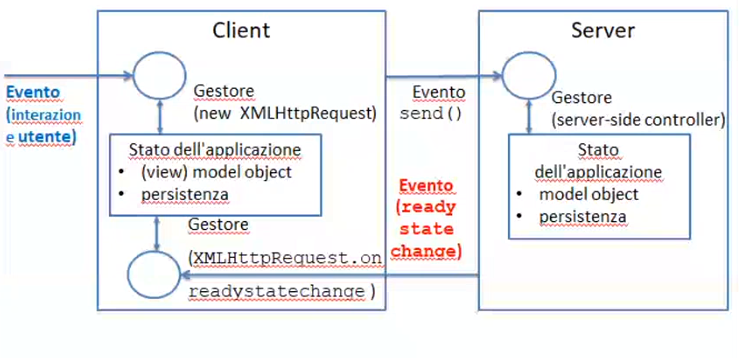
\includegraphics[height=4cm]{../lezione18/img1.PNG}
\end{center}
Notiamo che ora la nostra applicazione a lato client deve gestire due fonti di eventi: quelle dell'utente e quelle del server (readystatechange).\newline
Vediamo ora un'immagine che mostra l'architettura complessiva:
\begin{center}
    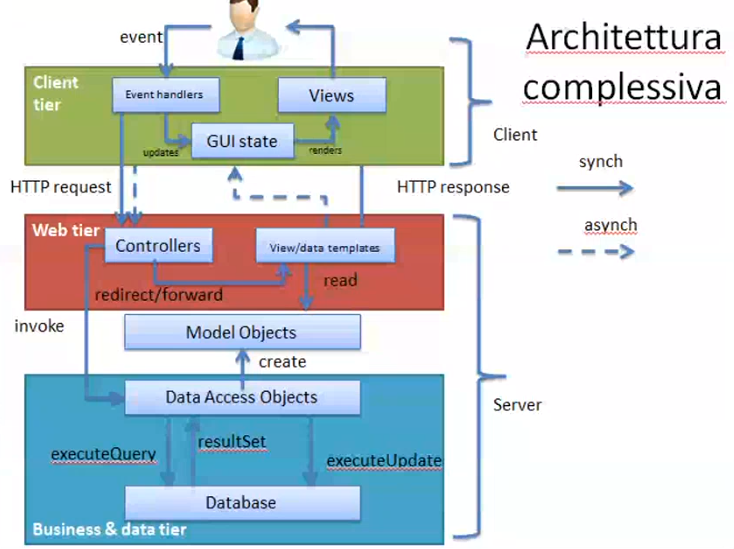
\includegraphics[height=3cm]{../lezione18/img2.PNG}
\end{center}